%!TEX program = xelatex
\documentclass[dvipsnames, svgnames,a4paper,11pt]{article}
% ----------------------------------------------------
%   中山大学物理与天文学院本科实验报告模板
%   作者:Huanyu Shi,2019级
%   知乎:https://www.zhihu.com/people/za-ran-zhu-fu-liu-xing
%   Github:https://github.com/huanyushi/SYSU-SPA-Labreport-Template
%   Last update : 2023.4.10
% ----------------------------------------------------

% ----------------------------------------------------- 
%	加边框的命令
%	参考:https://tex.stackexchange.com/questions/531559/how-to-add-the-page-border-for-first-two-pages-in-latex
\usepackage{tikz}
\usetikzlibrary{calc}
\usepackage{eso-pic}
\AddToShipoutPictureBG{%
\begin{tikzpicture}[overlay,remember picture]
\draw[line width=0.6pt] % 边框粗细
    ($ (current page.north west) + (0.6cm,-0.6cm) $)
    rectangle
    ($ (current page.south east) + (-0.6cm,0.6cm) $); % 边框位置
\end{tikzpicture}}


\usepackage{xcolor}
\definecolor{c1}{HTML}{2752C9} % 目录颜色
\definecolor{c2}{RGB}{190,20,83} % 引用颜色

\usepackage{ctex}
\usepackage[top=28mm,bottom=28mm,left=15mm,right=15mm]{geometry}
\usepackage{hyperref} 
\hypersetup{
	colorlinks,
	linktoc = section, % 超链接位置,选项有section, page, all
	linkcolor = c1, % linkcolor 目录颜色
	citecolor = c1  % citecolor 引用颜色
}
\usepackage{amsmath,enumerate,multirow,float}
\usepackage{tabularx}
\usepackage{tabu}
\usepackage{subfig}
\usepackage{fancyhdr}
\usepackage{graphicx}
\usepackage{wrapfig}  
\usepackage{physics}
\usepackage{appendix}
\usepackage{amsfonts}

%
\usepackage{tcolorbox}
\tcbuselibrary{skins,breakable}
\newtcolorbox{tbox}[2][]{
    colframe=black!70!,
    breakable,
    enhanced,
	boxrule =0.5pt,
    title = {#2},
    fonttitle = \large\kaishu\bfseries,
	drop fuzzy shadow,
    #1
}
\newtcolorbox[auto counter,number within=section]{question}[1][]{
  top=2pt,bottom=2pt,arc=1mm,
  boxrule=0.5pt,
%   frame hidden,
  breakable,
  enhanced, %跨页后不会显示下边框
  coltitle=c1!80!gray,
  colframe=c1,
  colback=c1!3!white,
  drop fuzzy shadow,
  title={思考题~\thetcbcounter:\quad},
  fonttitle=\bfseries,
  attach title to upper,
  #1
}

% ---------------------------------------------------------------------
%	利用cleveref改变引用格式,\cref是引用命令
\usepackage{cleveref}
\crefformat{figure}{#2{\textcolor{c2}{图 #1}}#3} % 图片的引用格式
\crefformat{equation}{#2{(\textcolor{c2}{#1})}#3} % 公式的引用格式
\crefformat{table}{#2{\textcolor{c2}{表 #1}}#3} % 表格的引用格式


% ---------------------------------------------------------------------
%	页眉页脚设置
\fancypagestyle{plain}{\pagestyle{fancy}}
\pagestyle{fancy}
\lhead{\kaishu 中山大学物理与天文学院近代物理实验\uppercase\expandafter{\romannumeral1}} % 左边页眉,学院 + 课程
\rhead{\kaishu D8 \quad 氦氖激光综合实验} % 右边页眉,实验报告标题
\cfoot{\thepage} % 页脚,中间添加页码


% ---------------------------------------------------------------------
%	对目录、章节标题的设置
\renewcommand{\contentsname}{\centerline{\huge 目录}}
\usepackage{titlesec}
\usepackage{titletoc}
% \titleformat{章节}[形状]{格式}{标题序号}{序号与标题间距}{标题前命令}[标题后命令]
\titleformat{\section}{\centering\LARGE\songti}{}{1em}{}

% ---------------------------------------------------------------------
%   listing代码环境设置
\usepackage{listings}
\lstloadlanguages{python}
\lstdefinestyle{pythonstyle}{
backgroundcolor=\color{gray!5},
language=python,
frameround=tftt,
frame=shadowbox, 
keepspaces=true,
breaklines,
columns=spaceflexible,                   
basicstyle=\ttfamily\small, % 基本文本设置,字体为teletype,大小为scriptsize
keywordstyle=[1]\color{c1}\bfseries, 
keywordstyle=[2]\color{Red!70!black},   
stringstyle=\color{Purple},       
showstringspaces=false,
commentstyle=\ttfamily\scriptsize\color{green!40!black},%注释文本设置,字体为sf,大小为smaller
tabsize=2,
morekeywords={as},
morekeywords=[2]{np, plt, sp},
numbers=left, % 代码行数
numberstyle=\it\tiny\color{gray}, % 代码行数的数字字体设置
stepnumber=1,
rulesepcolor=\color{gray!30!white}
}




% ---------------------------------------------------------------------
%	其他设置
\def\degree{${}^{\circ}$} % 角度
\graphicspath{{./images/}} % 插入图片的相对路径
\allowdisplaybreaks[4]  %允许公式跨页 % 导入模板的相关设置
\usepackage{lipsum}
\usepackage{enumitem}
\usepackage{tabularray}  %绘制表格时可以更加方便添加框线
\usepackage{longtable}
\setlist[enumerate]{label=\textup{(\arabic*)}}



%---------------------------------------------------------------------
%	正文
%---------------------------------------------------------------------

\begin{document}


\begin{table}
	\renewcommand\arraystretch{1.7}
	\begin{tabularx}{\textwidth}{
		|X|X|X|X
		|X|X|X|X|}
	\hline
	\multicolumn{2}{|c|}{预习报告}&\multicolumn{2}{|c|}{实验记录}&\multicolumn{2}{|c|}{分析讨论}&\multicolumn{2}{|c|}{总成绩}\\
	\hline
	\LARGE25 & & \LARGE30 & & \LARGE25 & & \LARGE80 & \\
	\hline
	\end{tabularx}
\end{table}


\begin{table}
	\renewcommand\arraystretch{1.7}
	\begin{tabularx}{\textwidth}{|X|X|X|X|}
	\hline
	专业:& 物理学 &年级:& 2022级\\
	\hline
	姓名:& 戴鹏辉  & 学号: & 2344016 \\
	\hline
	日期:& 2024/10/14 & 教师签名:& \\
	\hline
	\end{tabularx}
\end{table}

\begin{center}
	\LARGE D8 \quad 氦氖激光综合实验
\end{center}

\textbf{【实验报告注意事项】}
\begin{enumerate}
	\item 实验报告由三部分组成:
	\begin{enumerate}
		\item 预习报告:(提前一周)认真研读\underline{\textbf{实验讲义}},弄清实验原理;实验所需的仪器设备、用具及其使用(强烈建议到实验室预习),完成课前预习思考题;了解实验需要测量的物理量,并根据要求提前准备实验记录表格(第一循环实验已由教师提供模板,可以打印)。预习成绩低于10分(共20分)者不能做实验。
	    \item 实验记录:认真、客观记录实验条件、实验过程中的现象以及数据。实验记录请用珠笔或者钢笔书写并签名(\textcolor{red}{\textbf{用铅笔记录的被认为无效}})。\textcolor{red}{\textbf{保持原始记录,包括写错删除部分,如因误记需要修改记录,必须按规范修改。}}(不得输入电脑打印,但可扫描手记后打印扫描件);离开前请实验教师检查记录并签名。
	    \item 分析讨论:处理实验原始数据(学习仪器使用类型的实验除外),对数据的可靠性和合理性进行分析;按规范呈现数据和结果(图、表),包括数据、图表按顺序编号及其引用;分析物理现象(含回答实验思考题,写出问题思考过程,必要时按规范引用数据);最后得出结论。
	\end{enumerate}
	\textbf{实验报告就是将预习报告、实验记录、和数据处理与分析合起来,加上本页封面。}
	% \item 每次完成实验后的一周内交\textbf{实验报告}(特殊情况不能超过两周)。
	\item 实验报告注意事项
		\begin{enumerate}[label=\roman*.]
			\item \textbf{务必避免激光直射入眼,各小组务必保证本组所用激光不能射出本小组所用
			实验台。}
			\item 请勿随意拆卸光路中已经固定的器件。
			\item 实验过程,请保持站立,请勿落座。
			\item 操作光机组件,请勿大力扭摆,请勿用手接触器件表面。
			\item 使用功率计时注意不要使激光功率超过功率计量程。
			\item 激光器、法布里-珀罗干涉仪、功率计使用和维护参考相应用户手册指导。
			\item 注意一定在相机前插入衰减片,防止强光损坏相机。
		\end{enumerate}
\end{enumerate}


\clearpage
\tableofcontents
\clearpage

\setcounter{section}{0}
\section{D8 \quad 氦氖激光综合实验 \quad\heiti 预习报告}
	
\subsection{实验目的}
\begin{enumerate}
	\item 理解激光谐振原理,掌握激光谐振腔的调节方法,学会测量激光光斑功率大小;
	\item 了解激光器的纵模与横模的区别,掌握测量和改变激光器纵模的方法;
	\item 理解激光光束特性的主要参数,掌握激光传播特性的主要参数的测量方法;
	\item 了解激光光束变换的原理,掌握对高斯光束的变换与测量。
	
\end{enumerate}

\subsection{仪器用具}

% \begin{table}[htbp]
% 	\centering
% 	\renewcommand\arraystretch{1.6}
% 	% \setlength{\tabcolsep}{10mm}
% 	\caption{偏振测量实验}
% 	\begin{tabular}{p{0.05\textwidth}|p{0.20\textwidth}|p{0.5\textwidth}|p{0.05\textwidth}}
% 		\hline
% 		编号& 仪器用具名称  &  主要参数(型号,测量范围,测量精度等)& 数量 \\
% 		\hline
% 		1	&	法布里-珀罗干涉仪 	& 波长 633nm,精细常数大于 100,3.75G & 1 \\

% 		2	&	氦氖内腔激光器 	& 633nm,P>1.5mW,TEM00 & 1	 \\
		
% 		3	&	氦氖半外腔激光管 & 半外腔 250 激光管,含 3 个腔片 &	1 	\\
		
% 		4	&	氦氖半外腔激光器	& 半外腔,633nm,>1.5mW,TEM00 & 1	\\
		
% 		5	&	激光功率计	& 100nW-100mW 测试范围 & 1	\\

% 		6	&	CMOS 相机	& 120 万像素,黑白,1292×964,3.75um 像素,1/3 & 1 \\

% 		7	&	钢尺	& 500mm & 1	\\

% 		8	&	激光器电源部件	&  & 1	\\

% 		9	&	白屏(带刻度)	& 外形 210×150×2mm,单面带一维刻度 & 1	\\

% 		10	&	窗口 	& Φ25.4mm,T=2mm,0.2\%透过率,装在转接座中 & 1	\\

% 		11	&	窗口	& Φ25.4mm,T=2mm,10\%透过率,装在转接座中  & 1	\\

% 		12	&	窗口	& Φ25.4mm,T=2mm,2\%透过率,装在转接座中  & 1	\\

% 		13	&	窗口	& Φ25.4mm,T=4mm,装在相机转接座中  & 1	\\

% 		14	&	可变光阑	& 通光 Φ2~Φ28mm,外径 Φ50mm  & 1	\\

% 		15	&	平凸透镜	& Φ25.4mm,f75mm,装在 Φ25.4 透镜/反射镜座中  & 1	\\

% 		16	&	双凸透镜	& Φ40mm,f150mm,装在 Φ40 透镜/反射镜座中  & 1	\\

% 		17	&	相机转接座	& 装 Φ25.4mm 镜片,C 接口  & 1	\\

% 		18	&	转接座	& 装 Φ25.4mm 镜片  & 3	\\

% 		19	&	十字叉丝板	& 90×70×2mm,中心 Φ1mm 小孔  & 1	\\

% 		20	&	干板夹	& 外形 60×26×24mm  & 1	\\

% 		21	&	相机转接底板	& 转接水星相机与支杆  & 1	\\

% 		22	&	90mm 导轨	& 90mm 宽,30mm 高,1200mm 长  & 1	\\
		
% 		23	&	90mm 滑块	& 120mm 宽,40mm 长  & 2	\\

% 		24	&	90mm Y 向移动滑块	& 120mm 宽,40mm 长,Y 轴平移  & 2	\\

% 		25	&	调节套筒	& L76mm  & 6	\\

% 		26	&	支杆	& L76mm,双头阳螺纹  & 4	\\

% 		27	&	激光管夹持器	& Φ25~Φ50mm,V 型  & 2	\\

% 		\hline
% 	\end{tabular}
% 	\label{tbl:偏振测量实验}
% \end{table}


\begin{longtable}{p{0.05\textwidth}|p{0.20\textwidth}|p{0.5\textwidth}|p{0.05\textwidth}}
	\caption{氦氖激光综合实验实验用具}\\
	\hline
	编号 & 仪器用具名称 & 主要参数(型号,测量范围,测量精度等) & 数量 \\
	\hline
	\endfirsthead

	\multicolumn{4}{c}%
	{氦氖激光综合实验实验用具(续前页)} \\
	\hline
	编号 & 仪器用具名称 & 主要参数(型号,测量范围,测量精度等) & 数量 \\
	\hline
	\endhead

	\hline \multicolumn{4}{r}{继续下页} \\
	\endfoot

	\hline
	\endlastfoot

	1 & 法布里-珀罗干涉仪 & 波长 633nm,精细常数大于 100,3.75G & 1 \\

	2 & 氦氖内腔激光器 & 633nm,P>1.5mW,TEM00 & 1	 \\

	3 & 氦氖半外腔激光管 & 半外腔 250 激光管,含 3 个腔片 &	1 	\\

	4 & 氦氖半外腔激光器 & 半外腔,633nm,>1.5mW,TEM00 & 1	\\

	5 & 激光功率计 & 100nW-100mW 测试范围 & 1	\\

	6 & CMOS 相机 & 120 万像素,黑白,1292×964,3.75um 像素,1/3 & 1 \\

	7 & 钢尺 & 500mm & 1	\\

	8 & 激光器电源部件 &  & 1	\\
	
	9 & 白屏(带刻度) & 外形 210×150×2mm,单面带一维刻度 & 1	\\

	10 & 窗口 & Φ25.4mm,T=2mm,0.2\%透过率,装在转接座中 & 1	\\

	11 & 窗口 & Φ25.4mm,T=2mm,10\%透过率,装在转接座中  & 1	\\

	12 & 窗口 & Φ25.4mm,T=2mm,2\%透过率,装在转接座中  & 1	\\

	13 & 窗口 & Φ25.4mm,T=4mm,装在相机转接座中  & 1	\\

	14 & 可变光阑 & 通光 Φ2~Φ28mm,外径 Φ50mm  & 1	\\

	15 & 平凸透镜 & Φ25.4mm,f75mm,装在 Φ25.4 透镜/反射镜座中  & 1	\\

	16 & 双凸透镜 & Φ40mm,f150mm,装在 Φ40 透镜/反射镜座中  & 1	\\

	17 & 相机转接座 & 装 Φ25.4mm 镜片,C 接口  & 1	\\

	18 & 转接座 & 装 Φ25.4mm 镜片  & 3	\\

	19 & 十字叉丝板 & 90×70×2mm,中心 Φ1mm 小孔  & 1	\\

	20 & 干板夹 & 外形 60×26×24mm  & 1	\\

	21 & 相机转接底板 & 转接水星相机与支杆  & 1	\\

	22 & 90mm 导轨 & 90mm 宽,30mm 高,1200mm 长  & 1	\\

	23 & 90mm 滑块 & 120mm 宽,40mm 长  & 2	\\

	24 & 90mm Y 向移动滑块 & 120mm 宽,40mm 长,Y 轴平移  & 2	\\

	25 & 调节套筒 & L76mm  & 6	\\
	
	26 & 支杆 & L76mm,双头阳螺纹  & 4	\\

	27 & 激光管夹持器 & Φ25~Φ50mm,V 型  & 2	\\
\end{longtable}




% \clearpage

\subsection{原理概述}

	\begin{enumerate}
		\item \textbf{氦氖激光器谐振腔虚拟仿真和调整实验:}

			He-Ne激光器是一种激光设备,由光学谐振腔、工作物质和激励系统组成。工作物质是密封在玻璃管中的氦气和氖气,当这些气体被电流激励时,会在特定能级上产生粒子数反转,形成增益介质。增益介质的增益特性与毛细管的长度、内径、气体比例、总气压和放电电流等因素密切相关。光学谐振腔的设计要满足频率的驻波条件和腔的稳定条件,以确保激光波长与腔长匹配,并且腔镜的曲率半径合适,以保证激光能在腔内稳定传播。只有当谐振腔的损耗小于介质的增益时,激光振荡才能建立起来,从而产生激光。

			下面计算氦氖激光中单模激光器的输出功率:

			激光稳定后,其饱和增益系数应等于总损耗系数,即:
			\[
				G(v, I_v) = a - \frac{1}{2l} \ln(R_1 R_2)
			\]
			$a$为除反射镜损耗外其他的总损耗系数,$l$为放电管长度,$R_1, R_2$为两反射镜的反射率。

			一般情况下,He-Ne 激光器的一端为全反射,另一端为部分反射,设透过率为$T$,忽略反射镜的吸收和散射损耗时,$R_2 = 1 - T$。由于 He-Ne 激光器的 $T$ 和 $a$ 都很小,则有:
			\begin{align}
				-\ln(R_1 R_2) = -\ln(1 - T ) \approx T	\nonumber \\
				a_c = 1 - e^{-2al} \approx 2al	\nonumber
			\end{align}

			$a_c$是除透射损耗外,光在谐振腔内往返一次的总损耗百分数。
			
			做近似代换后得到:$\Rightarrow 2 G(v, I_v) l = a_c + T $

			引入激发参量 $\beta = 2 G_m l / (a_c + T)$。由$\beta$能图解法计算出$I_{v0}$ ,再根据下式计算出输出功率 $P$ ,其中$A$ 为光束的有效横截面积:
			\[
				P = A T I_{v0}^+
			\]

			


		\item \textbf{激光横模变换与参数测量实验:}
			
			激光的每一个频率对应一种光场分布,则模式。纵模描述轴向光场分布状态,横模描述横向分布状态。

			光在谐振腔中来回反射时,由于工作物质的横截面积和镜面都是有限的,当平行光通过它们时,因为衍射作用,使出射光波阵面发生畸变,从而在垂直于光的传播方向及横向上,将出现各种不同的场强分布,每一种分布形式叫做一种横模。

			横向分布是二维的,用三个指标 m、n、q 来完整的描述一个模式,m、n 代表横模序数,q 代表纵模序数。对同样的横模序数 m、n 有:
			\[
				\Delta \nu_{\text{纵}} = \frac{c}{2 \mu L} \Delta q
			\]

			对同一级 q,非共焦腔的横模频率差为:
			\[
				\Delta \nu_{\text{横}} = \frac{c}{2 \mu L} \{ \frac{1}{\pi} (\Delta m + \Delta n) \arccos[(1 - \frac{1}{R_1}) (1 - \frac{1}{R_2})]^{\frac{1}{2}} \}
			\]

			其中$\Delta m$ ,$\Delta n$ 分别表示$x$ ,$y$ 方向上横模模序数差,$R_1$,$R_2$ 为两反射镜的曲率半径,相邻横模频率间隔为
			\[
				\Delta \nu_{\Delta m + \Delta n = 1} = \Delta \nu_{\Delta q = 1} \{ \frac{1}{\pi} \arccos[(1 - \frac{L}{R_1})(1 - \frac{L}{R_2})]^{\frac{1}{2}} \}
			\]

			
		\item \textbf{高斯光束基本参数测量实验:}
		
			定态标量电磁场满足亥姆赫兹方程为
			\[
				\laplacian{E(\mathbf{r})} + k^2 E(\mathbf{r}) = 0
			\]
			
			在柱坐标下,高斯光束是亥姆赫兹方程在慢变振幅近似下的一个特解。高斯光束的电场为
			\[
				E(r, z) = A(r, z) e^{-ikz}
			\]
			其中
			\[
				A(r, z) = \frac{A_0 w_0}{w(z)} e^{-\frac{r^2}{w^2(z)}} e^{-i[\frac{k r^2}{2 R(z)} - \Psi]}
			\]

			高斯光束在任何一位置 $z$ 处的光强分布成均高斯形状。在径向方向 $r$ 为 $w(z)$处,光强减少至中心光强的 $1/e^2$。因此,上述定义的高斯光束半径常称为 $e$ 方分之一半径。高斯光束的光束半径随坐标 $z$ 按双曲线规律变化,即:
			\[
				\frac{w^2(z)}{w_0^2} - \frac{z^2}{z_0^2} = 1
			\]
			
			高斯光束有以下几个核心性质:高斯光束为截面光强呈高斯分布的光束。高斯光束的光束半径随坐标 z 呈双曲函数变化;在光腰位置的光束半径达到最小;在远场情况,高斯光束有近衍射极限的固定发散角。在旁轴情况下,光束的等相面为球面。在瑞利长度范围内,高斯光束可以近似为平行光和平面波。

			在测量光束传播参数时,沿光束传播轴,至少需要在十个不同位置上测量光斑直径,然后用双曲线拟合的方法求出光束参数。双曲线拟合方程为:$w^2(z) = A + B z + c z^2$ ($w(z)$为 $z$ 位置的束宽)。这些测量位置半数应位于束腰两侧一倍瑞利长度之内,其它测量位置在超过一倍瑞利长度之外。拟合求解出 $A$,$B$,$C$ 以后,可通过下表公式计算得到相应的光束参数:
			\begin{align}
				&\text{光腰位置:} z_0 = - \frac{B}{2C}	\nonumber	\\
				&\text{光腰半径:} \omega_0 = \sqrt{A - B^2/4C}	\nonumber	\\
				&\text{远场发散角:} \theta = \sqrt{C}	\nonumber	\\
				&\text{瑞利长度:} Z_0 = \frac{1}{2C} \sqrt{4AC - B^2}	\nonumber
			\end{align}


		\item \textbf{高斯光束的传播特性实验:}
		
			沿 z 轴传播的高斯光束的光场可以表示为以下形式
			\[
				E(r, z) = \frac{A_0 w_0}{w(z)} e^{-\frac{r^2}{w^2(z)}} e^{-i[\frac{k r^2}{2 R(z)} + k z - \Psi]} 
			\]

			可以使用复参数 q 来描述 z 处的高斯光束的性质。复参数 q 定义为
			\[
				\frac{1}{q(z)} = \frac{1}{R(z)} - i\frac{\lambda}{\pi w^2(z)}
			\]

			在高斯光束的传输问题中,可以用复参数 q 简洁地去描述高斯光束。

			高斯光束通过光学系统(如透镜)后的传播可以用ABCD矩阵来描述。这个矩阵可以用来计算光束经过光学系统后的q参数变化。
			
			若光束连续通过多个变换矩阵分别为 $M_1, M_2, M_3, …… , M_n$ 的光学元件组成的光学系统,则光学系统的总变换矩阵可以表示为每个独立元件的变换矩阵的乘积,即
			\[
				M = M_n …… M_3 M_2 M_1
			\]

			于是$q' = M q$

			% 当高斯光束通过焦距为$f$的薄透镜时,光束的束腰半径$w_0$和束腰位置$z_0$会发生变化。这些变化可以通过以下关系计算: 
			% \[
			% 	\frac{1}{w'^2} = \frac{1}{w_0^2} + \frac{2}{\lambda f^2} z' R' = z_0 R_0 + \frac{w_0^2}{f}
			% \]

			束腰半径是高斯光束所有光斑半径的最小值,可以将其类比为几何光学中光束的焦点,在满足近似假设条件的情况下,物方、像方高斯光束经过薄透镜后束腰位置和半径的变换规律与几何光学中的物、像规律相符,由此可见当满足条件时可以用几何光学的方法粗略的研究近轴高斯光束。当不满足近似条件时,则不能套用几何光学的结论。



	\end{enumerate}
	




\subsection{实验前思考题}

% 思考题1
\begin{question}
	氦氖激光器产生激光的原理是什么?它在哪些领域有应用?
\end{question}

	氦氖激光器的工作原理基于原子的受激辐射。在氦氖激光器中,工作物质是氦气和氖气的混合气体。当激光器工作时,放电管中的氦氖混合气体被电流激发,形成等离子体。在这个过程中,氦原子被激发到高能态,然后与氖原子发生碰撞,将能量传递给氖原子。

	氖原子获得能量后,会跃迁到更高的能级,但这些高能级是不稳定的,因此氖原子会很快跃迁回到较低的能级。在这个过程中,氖原子通过受激辐射的方式释放出光子。这些光子在激光器的谐振腔内来回反射,进一步激发更多的氖原子,产生更多的光子,形成一个连锁反应。由于谐振腔的作用,只有特定波长的光子能够持续在腔内来回反射并被放大,最终形成具有高度单色性、方向性和相干性的激光输出。

	在氦氖激光器中,最常见的激光输出波长为632.8纳米的红光,这个波长的激光是由于氖原子从3S能级跃迁到2P能级时产生的。此外,氦氖激光器还可以产生1.15微米和3.39微米的红外激光,但这些波长的激光输出功率通常较低。

	氦氖激光器的应用非常广泛,包括但不限于科学研究、精密测量、医疗治疗、工业加工和教育演示等。由于其激光具有高度的稳定性和单色性,它在需要精确光源的场合中尤为重要。
	


% 思考题2
\begin{question}
	请详细描述氦氖激光器的内部结构,包括哪些主要部件,并解释它们在激光产生过程中的作用。
\end{question}

	
	氦氖激光器的内部结构主要包括以下几个关键部件:

	\begin{enumerate}
		\item \textbf{放电管}:这是激光器的核心部分,通常由玻璃制成,内部充有氦氖混合气体。放电管内部的气压比约为5:1到10:1,总压强在133.3~266.6帕(1~2毫米汞柱)之间。放电管的阳极一般用钨棒制成,阴极为铝或钼圆筒。在放电过程中,氦原子被激发到高能态,然后与氖原子发生碰撞,将能量传递给氖原子,使得氖原子激发并最终产生激光。
		\item \textbf{谐振腔}:由两个反射镜组成,一个全反射镜和一个部分反射镜(输出耦合镜)。全反射镜位于激光器的一端,反射率非常高,通常超过99.99\%,而输出耦合镜位于另一端,具有一定透过率,通常约为1\%。这两个反射镜共同作用,使得光在腔内来回反射,从而实现光的放大和共振。
		\item \textbf{激励电源}:提供高压电能,用于激发放电管中的气体。电源将市用交流电转换为直流高压电,以维持气体放电所需的电能。氦氖激光器的启辉(点燃)电压通常高于工作电压,启辉电压约为4500V,工作电压约为1200V,最佳工作电流约为5mA。
		\item \textbf{窗口片}:在某些结构中,放电管两端会固定两块特殊的窗片,这些窗片与轴线呈一定倾角,使得反射镜可以安装在窗片外,便于调整以适应不同的实验要求。
	\end{enumerate}

	氦氖激光器的结构一般有三种形式:内腔式、外腔式和半内腔(或半外腔)式。内腔式激光器放电管与谐振腔固定在一起,使用方便,但稳定性较差。外腔式激光器放电管与谐振腔完全分开,腔体受温度影响较小,输出的激光为线偏振光,但使用不方便。半外腔式激光器则综合了前两种结构的优点,是一种比较理想的激光器。

	




% 思考题3
\begin{question}
	什么是横模和纵模?它们对激光束的特性分别有什么影响?
\end{question}

	横模和纵模是描述激光束特性的两个重要参数,它们分别描述了激光束在垂直于传播方向的横截面上的空间分布特性以及在沿传播方向上的频率分布特性。

	\begin{enumerate}
		\item \textbf{横模(Lateral Mode):}横模描述的是激光束在垂直于传播方向的横截面上的能量分布情况。它反映了激光束横截面的光强分布形状,通常用TEM(Transverse Electromagnetic)模式来表示。横模的编号如$TEM_{mn}$,其中m和n分别表示沿x和y方向的驻波节数。基模(Fundamental Mode)通常表示为$TEM_{00}$,它具有一个单一的、对称的光斑形状,且发散角最小,光束质量最好。高阶横模(Higher-Order Modes)在横截面上会有多个光斑,导致光束发散角增大,光束质量下降。横模的数量会影响激光器的光束质量,高阶模相比基模具有更大的发散角。
		
		\item \textbf{纵模(Longitudinal Mode):}纵模描述的是激光在谐振腔内形成的稳定驻波模式,与激光的频率或波长有关。对于一个固定的谐振腔,存在多个满足谐振条件的波长,每个波长对应一个纵模。单纵模激光器在腔内只有单个波长,而多纵模激光器则有多个波长。纵模的分布可以通过激光器的激射光谱来观察,通常在特定的波长范围内存在多个激射峰,这些激射峰对应的就是不同的纵模。谐振腔的腔长影响激光器的纵模数量,对于普通的垂直腔面发射激光器(VCSEL),由于腔长很短,通常都是单纵模输出。纵模决定了激光的频谱特性,影响激光的单色性。
	\end{enumerate}
	
	总的来说,横模影响激光束的空间特性,如光斑形状和发散角,而纵模影响激光束的频率特性,如单色性和光谱宽度。两者共同决定了激光束的质量和应用潜力。
	





% 思考题4
\begin{question}
	什么是 q 参数?它在高斯光束的描述中起什么作用?如何通过 q 参数计算高斯光束的束腰半径和等相位面曲率半径?
\end{question}

	q参数是高斯光束传播中的一个重要参数,它将描述高斯光束基本特征的两个参数——光束的束腰半径$\omega(z)$和等相位面的曲率半径$R(z)$——统一在一个表达式中。q参数的定义为:
	\[
		q(z) = \frac{\omega_0^2}{\lambda_z} + i z
	\]
	
	其中,$\omega_0$是束腰半径,$\lambda$是光波的波长,$z$是光束传播的距离,$i$是虚数单位。q参数有时也被称为高斯束的复曲率半径。

	q参数在高斯光束的描述中起着重要的作用,因为它可以用一个统一的公式来描述高斯光束通过自由空间及光学系统的行为。在自由空间中,高斯光束的传播规律可以用q参数来描述,形式上与普通球面波的传播规律相似。当高斯光束通过光学系统时,q参数的变换规律与普通球面波的曲率半径R的变换相同,这使得我们可以使用ABCD矩阵来描述高斯光束经过任意光学系统的变换。

	通过q参数,我们可以计算高斯光束的束腰半径和等相位面曲率半径。具体来说,如果我们知道某位置处的q参数值,就可以求出该位置处的$R(z)$和$\omega(z)$。例如,束腰半径$\omega(z)$可以通过下面的公式计算:
	\[
		\omega(z) = \omega_0 \sqrt{1 + (\frac{z}{z_R})^2}
	\]

	其中,$z_R$是瑞利距离,它与束腰半径$\omega_0$和波长$\lambda$的关系为:
	\[
		z_R = \frac{\pi \omega_0^2}{\lambda}
	\]

	等相位面的曲率半径$R(z)$可以通过下面的公式计算:
	\[
		R(z) = \frac{z}{\sqrt{1 - (\frac{z}{z_R})^2}}
	\]

	当$z$远小于$z_R$时,高斯光束可以近似看作是一束平行光,此时$R(z)$趋向于无穷大,$\omega(z)$近似等于$\omega_0$。随着$z$的增加,光束会发散,$R(z)$会减小,$\omega(z)$会增加。通过q参数,我们可以方便地研究高斯光束的传输特性和光学系统对光束的影响。






\clearpage
% \begin{table}
% 	\renewcommand\arraystretch{1.7}
% 	\centering
% 	\begin{tabularx}{\textwidth}{|X|X|X|X|}
% 	\hline
% 	专业:& 物理学 &年级:& 2022级 \\
% 	\hline
% 	姓名:& 戴鹏辉 & 学号:& 22344016 \\
% 	\hline
% 	室温:& 26℃ & 实验地点: & A413 \\
% 	\hline
% 	学生签名:& 
\includegraphics[width=0.9in]{name-TaLEs.jpg} & 评分: &\\
% 	\hline
% 	实验时间:& 2024/& 教师签名:&\\
% 	\hline
% 	\end{tabularx}
% \end{table}

\begin{table}
	\renewcommand\arraystretch{1.7}
	\centering
	\begin{tabularx}{\textwidth}{|X|X|X|X|}
	\hline
	专业:& 物理学 &年级:& 2022级 \\
	\hline
	姓名:& 戴鹏辉 & 学号:& 22344016 \\
	\hline
	室温:& 26℃ & 实验地点: & A413 \\
	\hline
	学生签名:& \raisebox{-0.5\height}{
\includegraphics[width=0.9in]{name-TaLEs.jpg}} & 评分: &\\
	\hline
	实验时间:& 2024/& 教师签名:&\\
	\hline
	\end{tabularx}
\end{table}



\section{D8 \quad 氦氖激光综合实验 \quad\heiti 实验记录}

\subsection{实验内容和步骤}



	\subsubsection{实验一 \quad 氦氖激光器谐振腔虚拟仿真和调整实验:}

		

	
	\subsubsection{实验二 \quad 激光横模变换与参数测量实验:}
	
	
		

	\subsubsection{实验三 \quad 高斯光束基本参数测量实验:}
	

		

	
	\subsubsection{实验四 \quad 高斯光束的传播特性实验:}

	


	\subsection{实验过程中遇到的问题记录}

		


\subsection{实验数据记录}

	% 见\cref{fig:data}

	% \begin{figure}[htbp]
	% 	\centering
	% 	% 第一行的三张图片
	% 	\subfloat[原始数据1]
	% 	{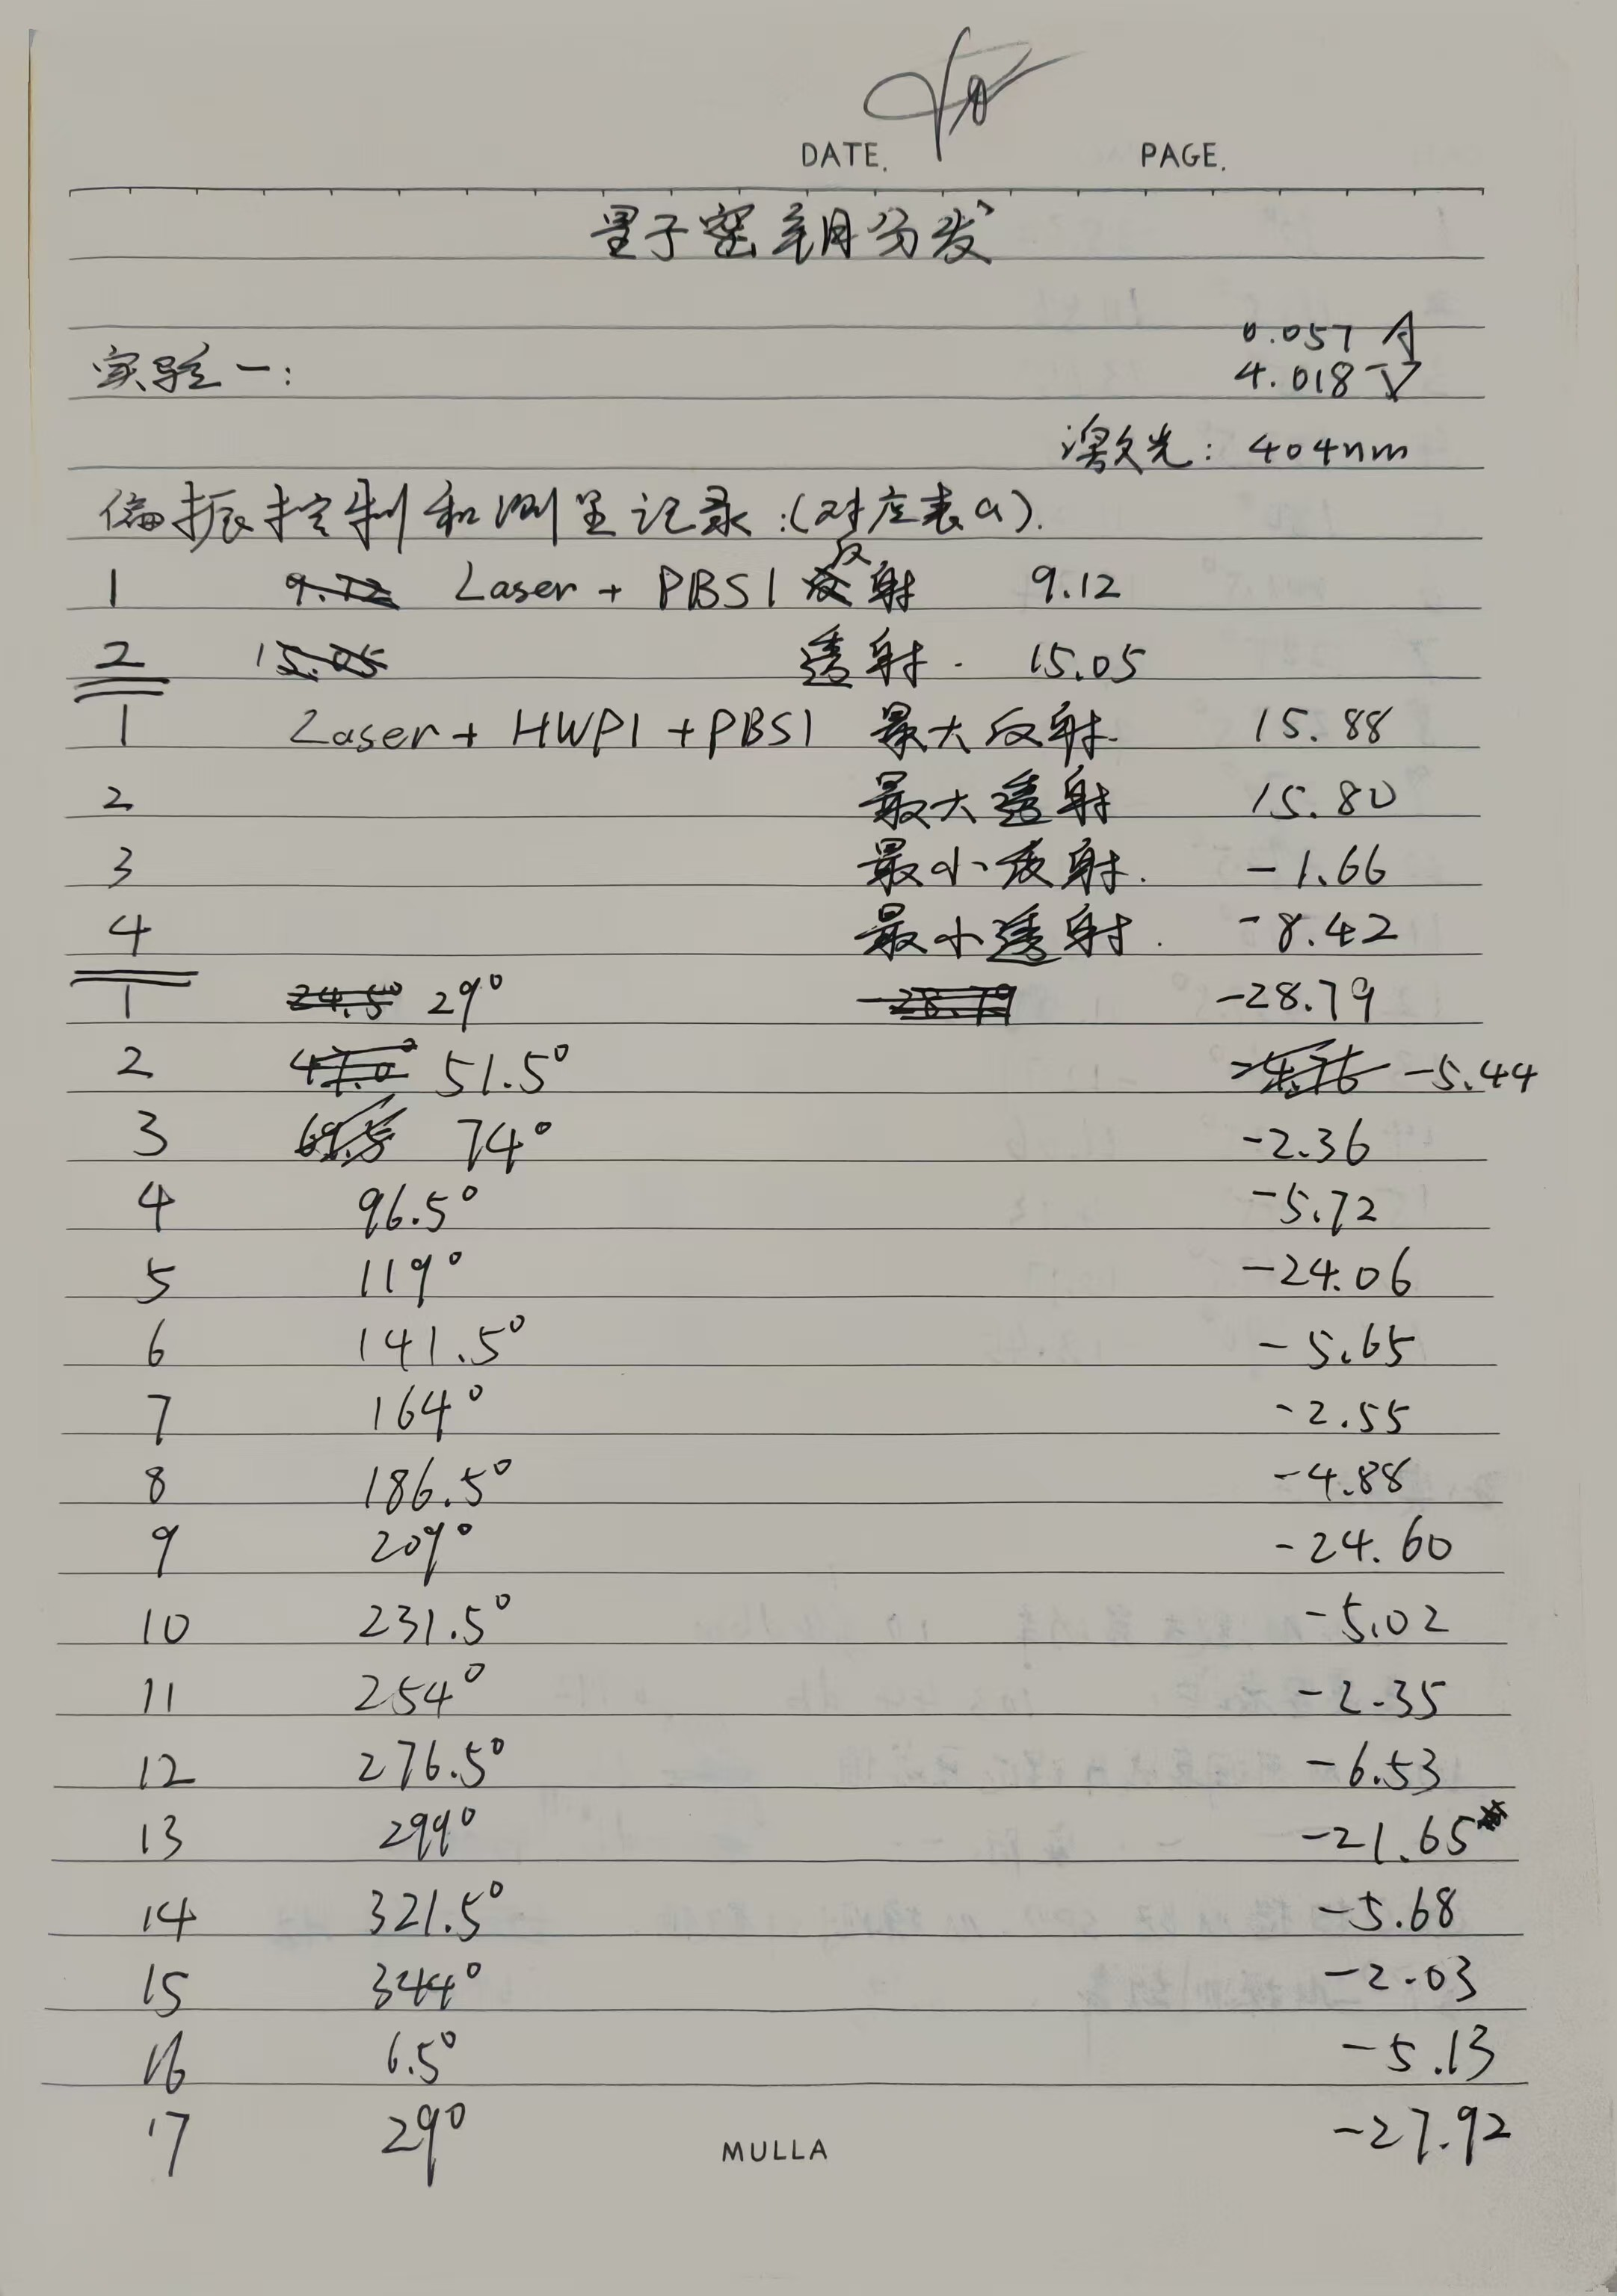
\includegraphics[width=0.3\textwidth]{D3-OriginalData-1.jpg}\label{fig:data1}}
	% 	\quad
	% 	\subfloat[原始数据2]
	% 	{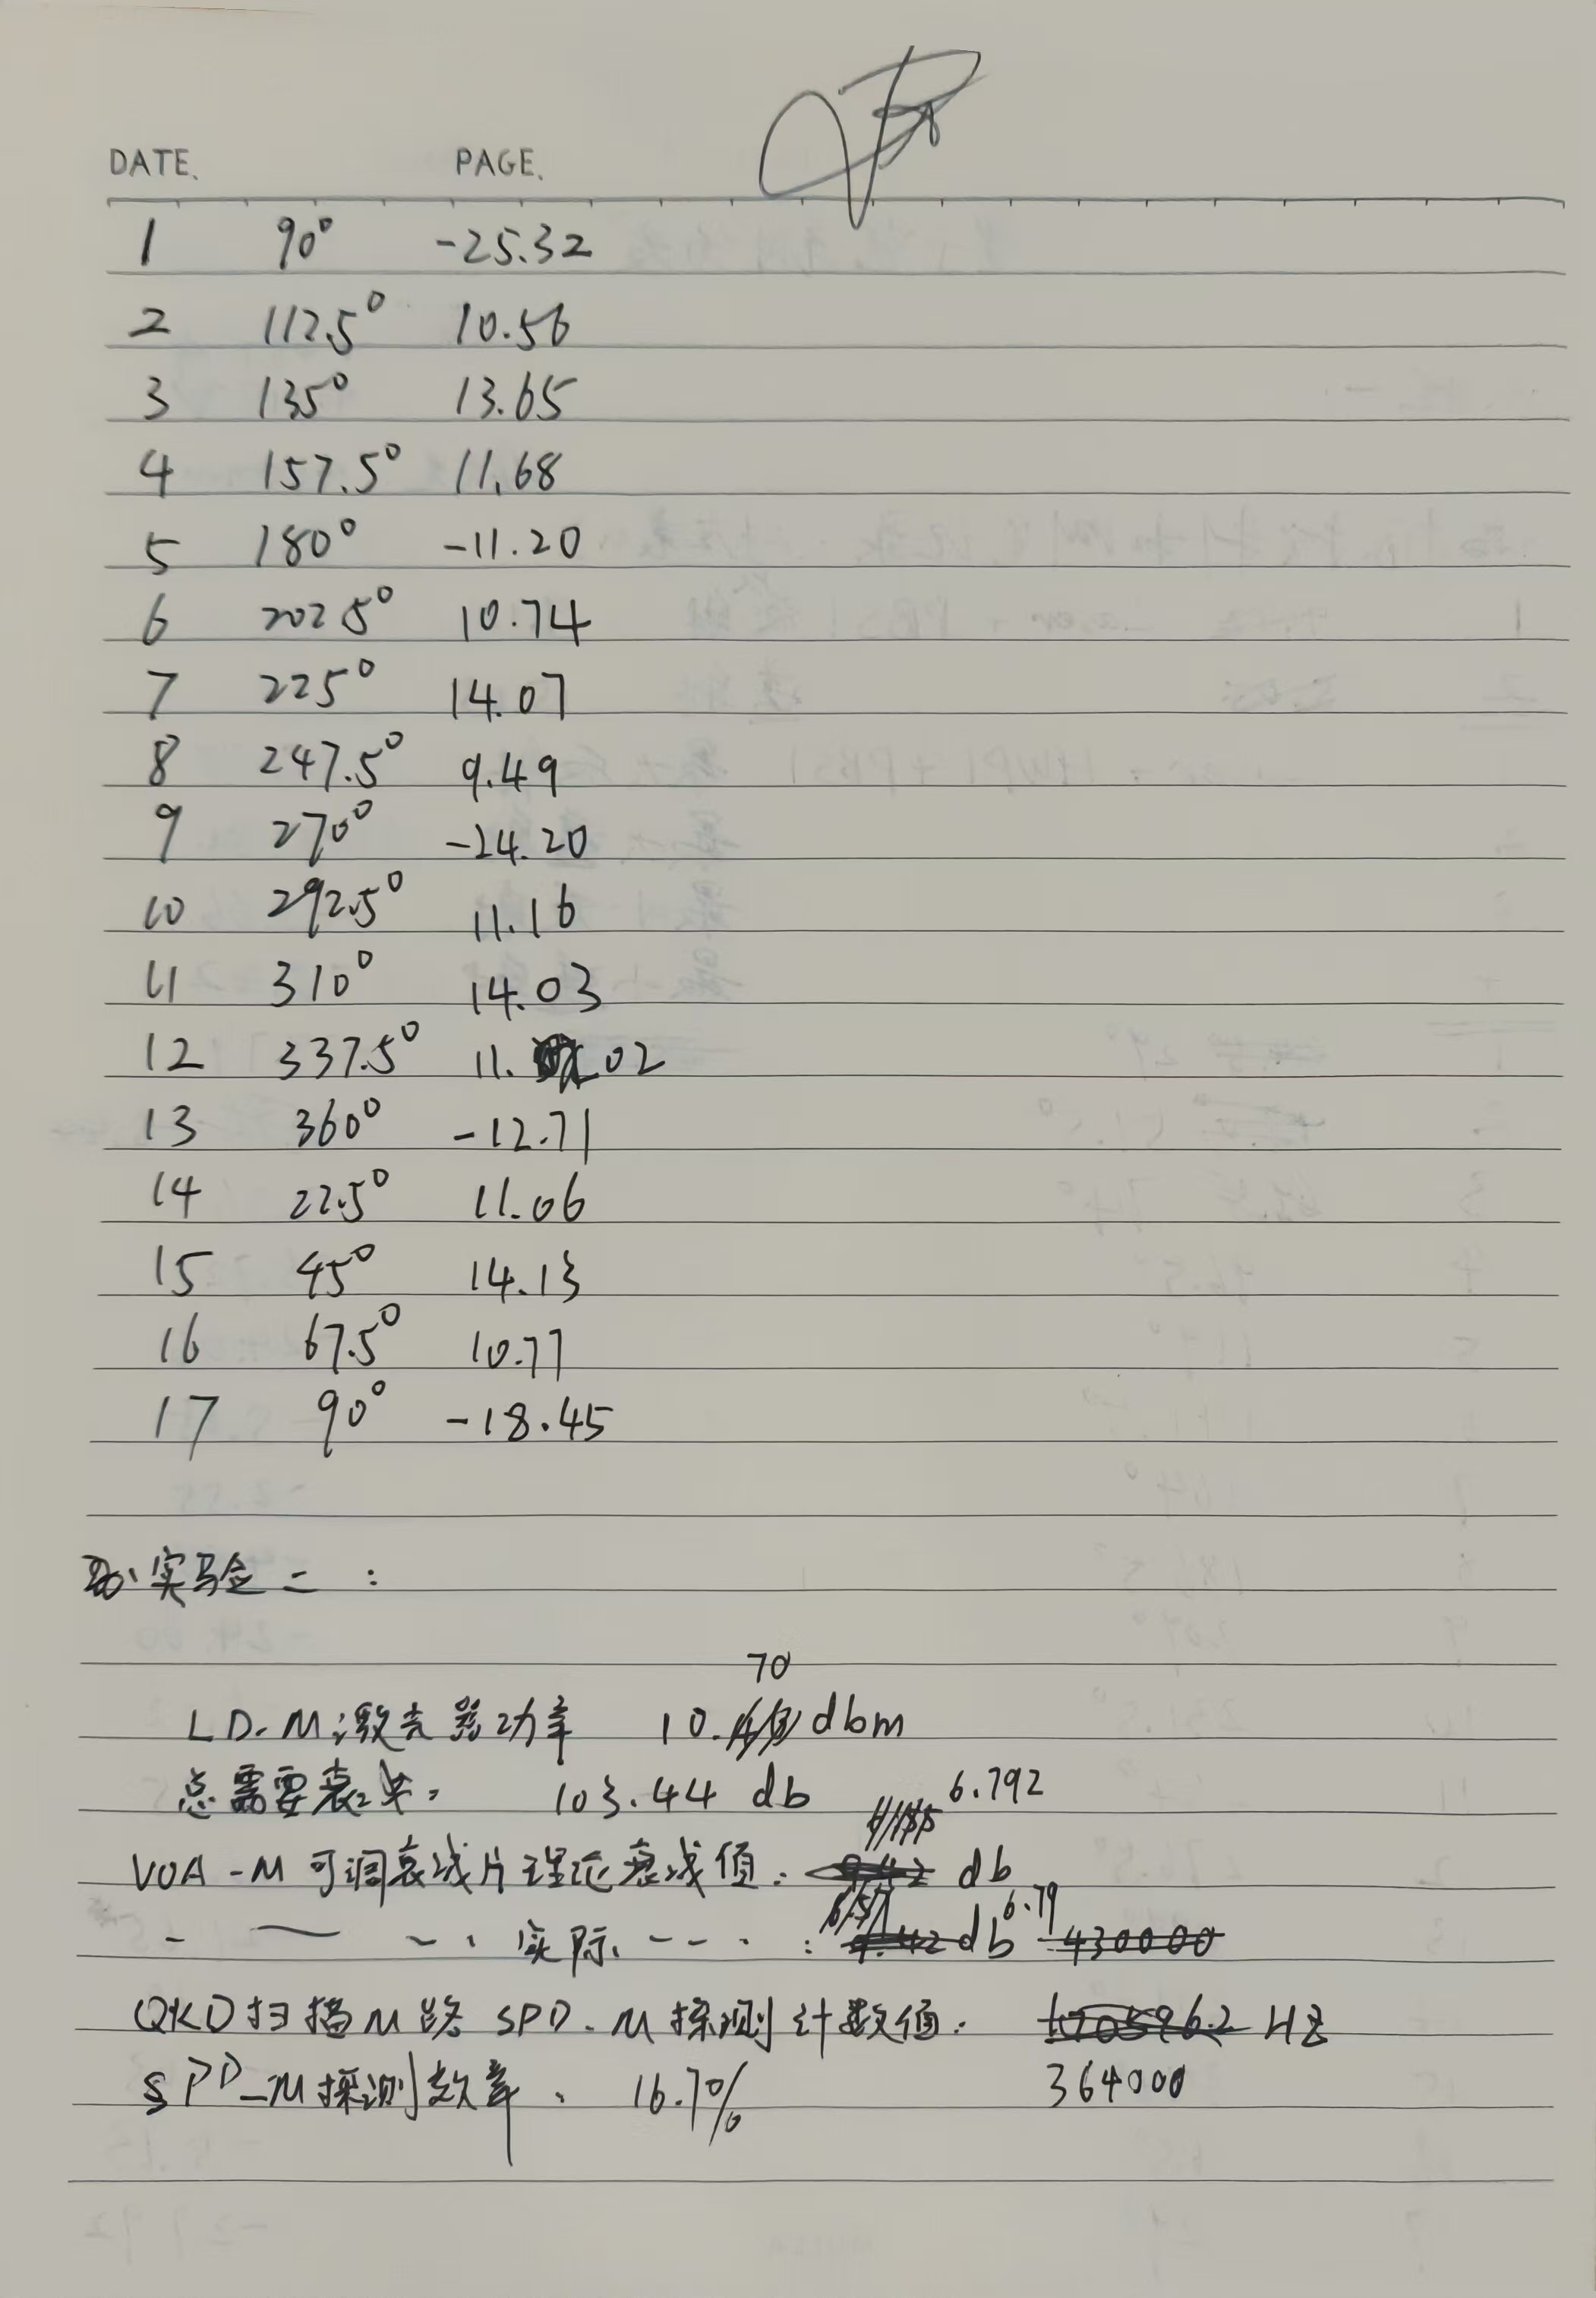
\includegraphics[width=0.3\textwidth]{D3-OriginalData-2.jpg}\label{fig:data2}}
	% 	\quad
	% 	\subfloat[原始数据3]
	% 	{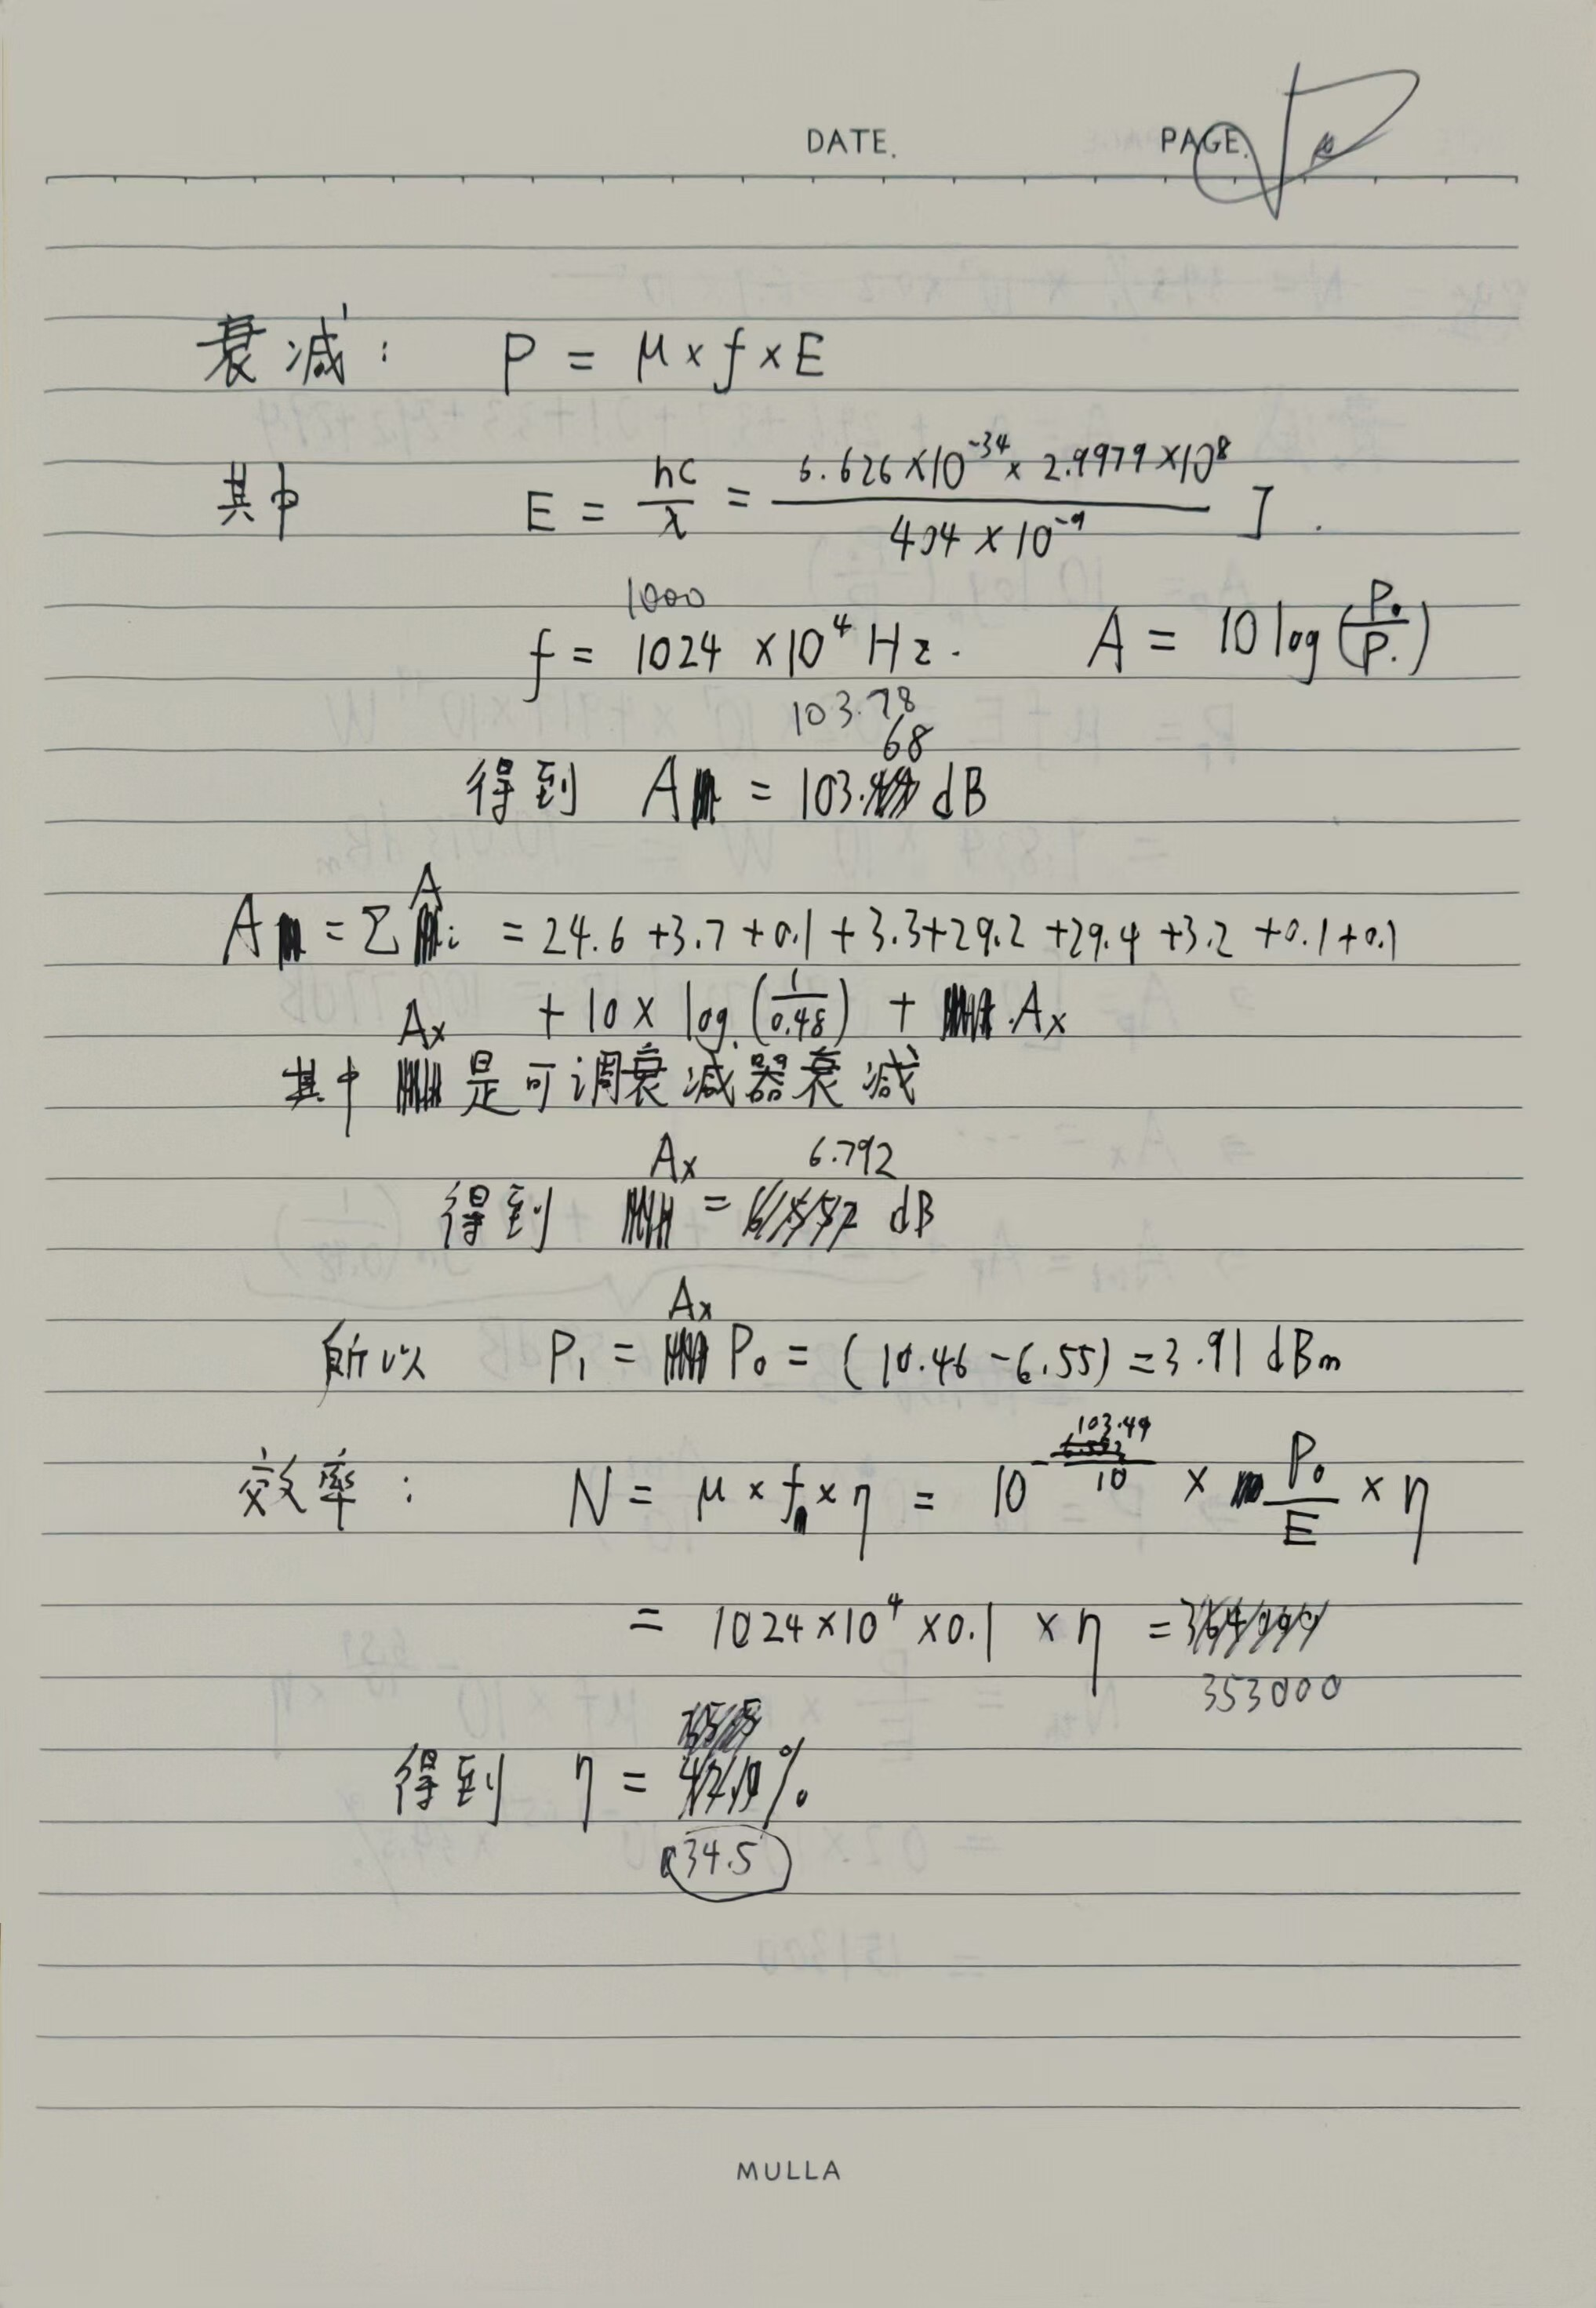
\includegraphics[width=0.3\textwidth]{D3-OriginalData-3.jpg}\label{fig:data3}}
	% 	\newline
	% 	% 第二行的两张图片
	% 	\subfloat[原始数据4]
	% 	{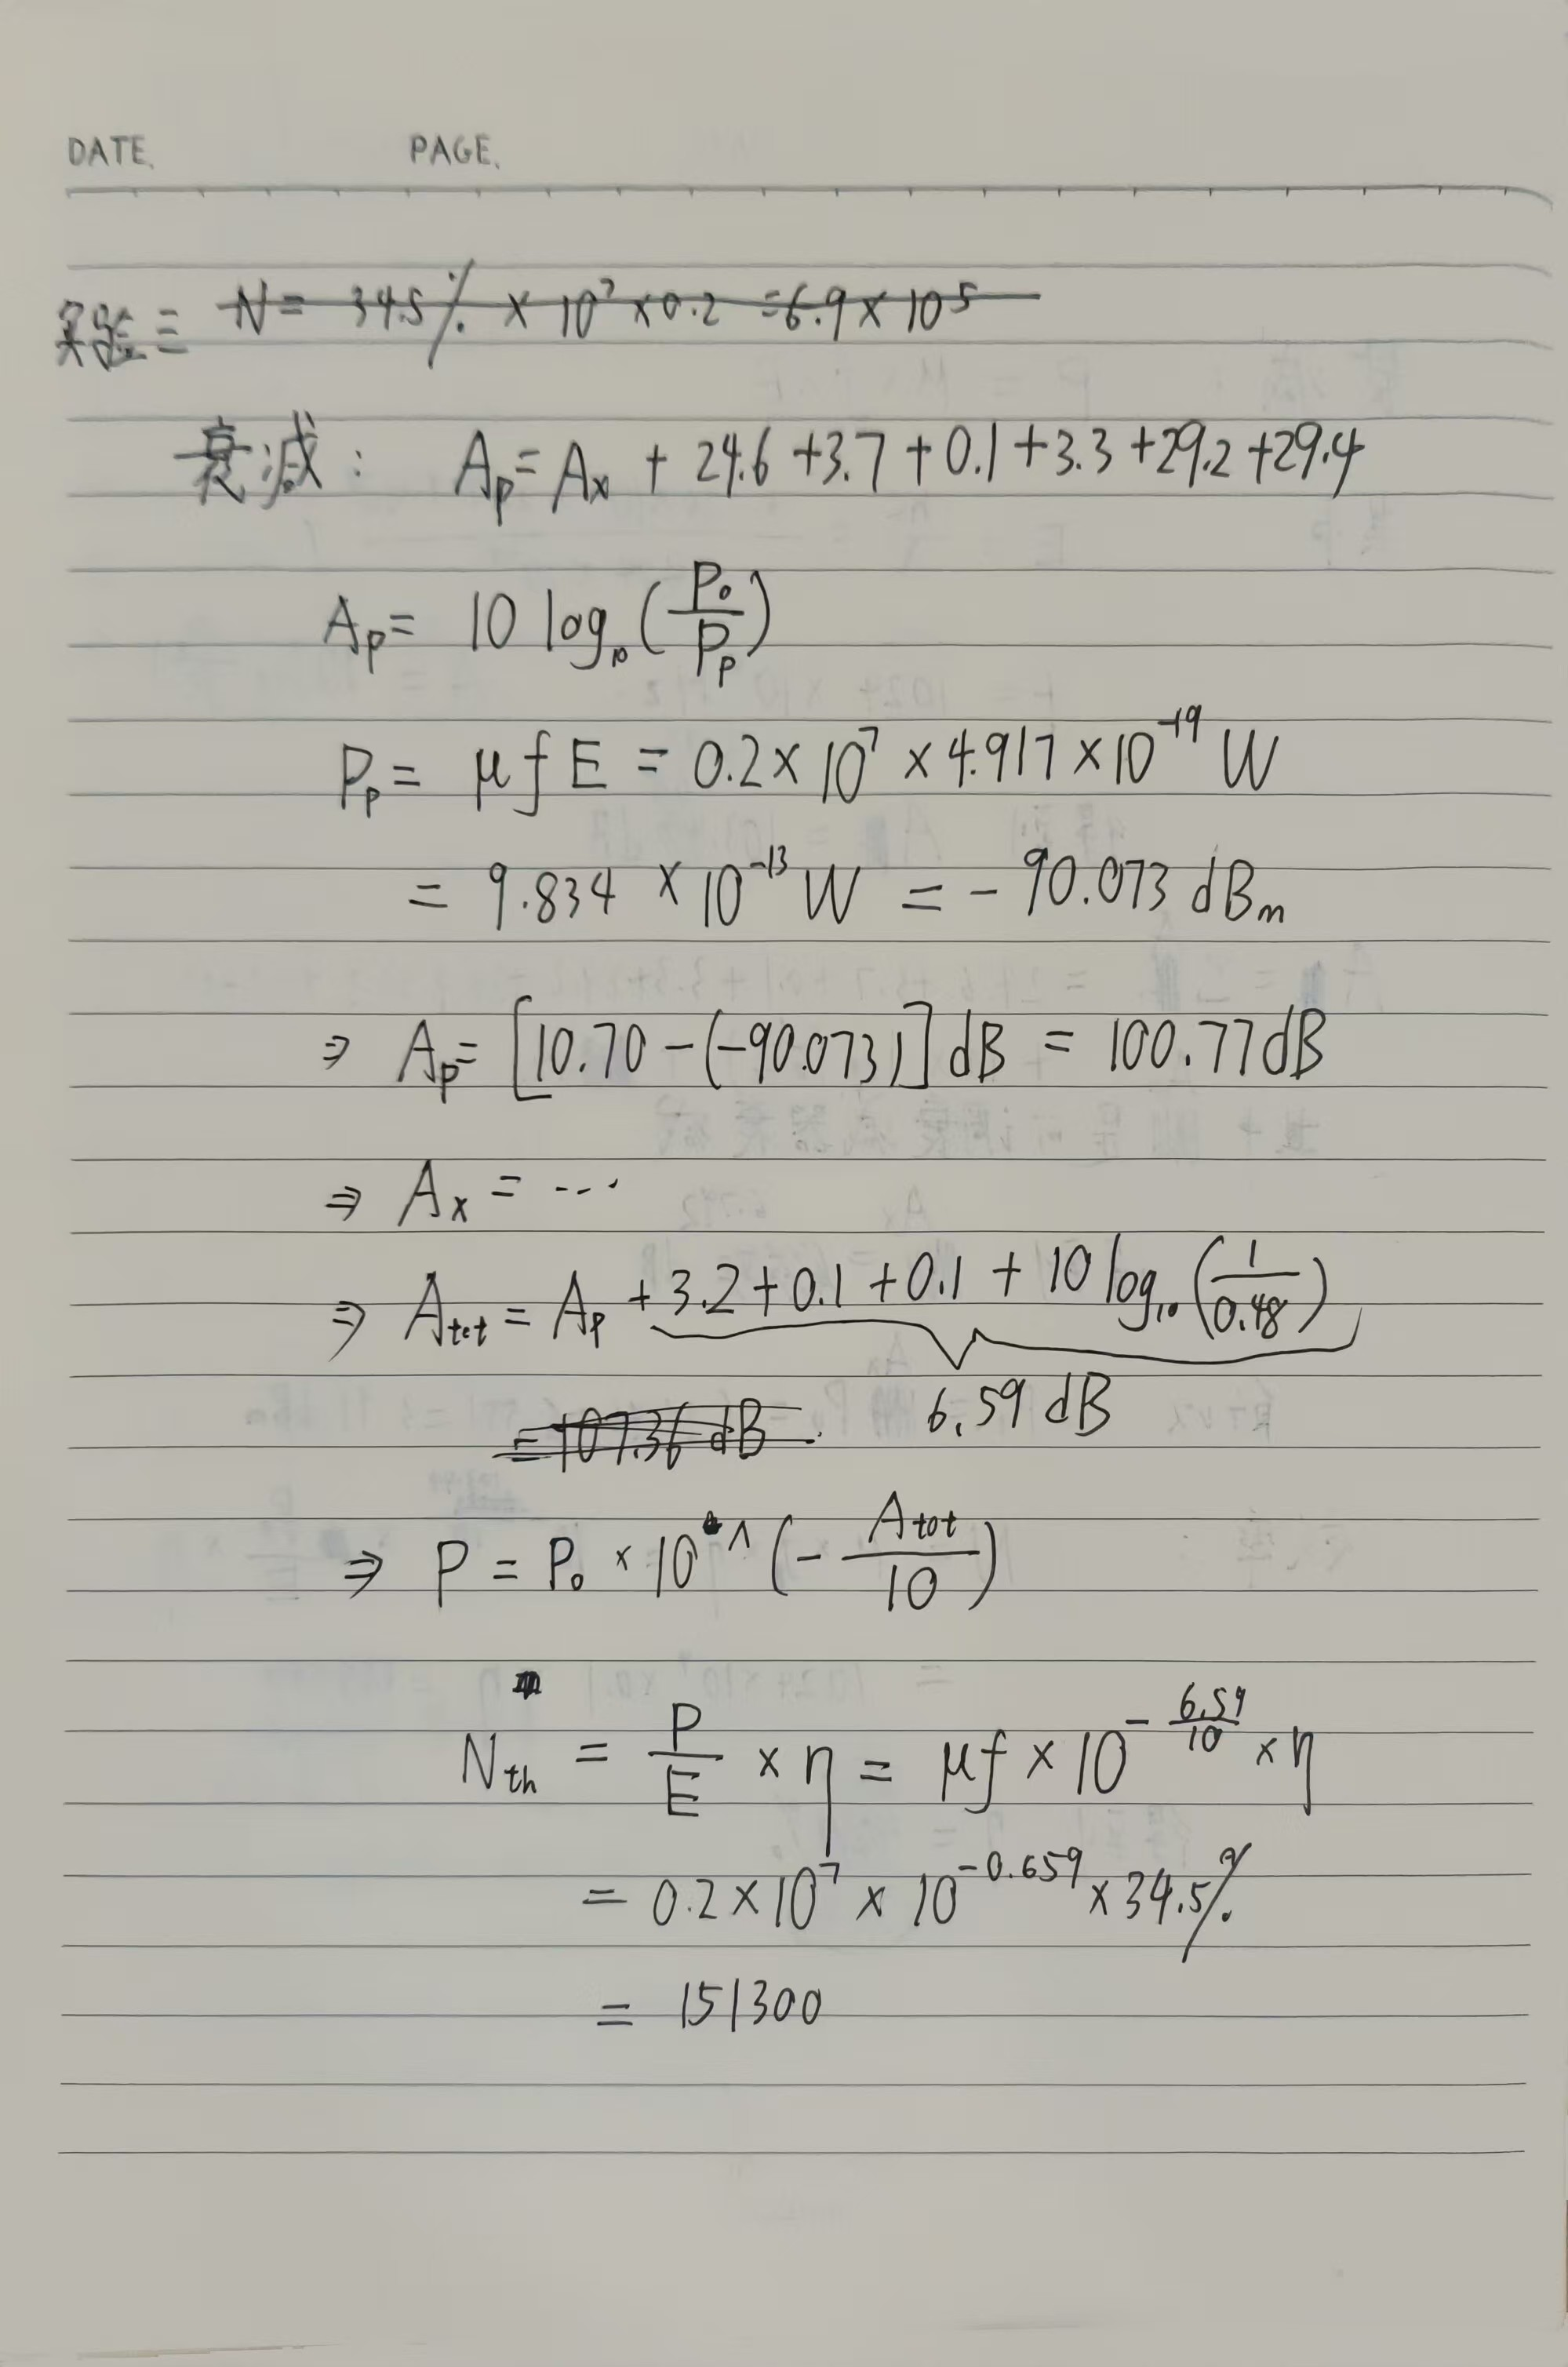
\includegraphics[width=0.3\textwidth]{D3-OriginalData-4.jpg}\label{fig:data4}}
	% 	\quad
	% 	\subfloat[原始数据5]
	% 	{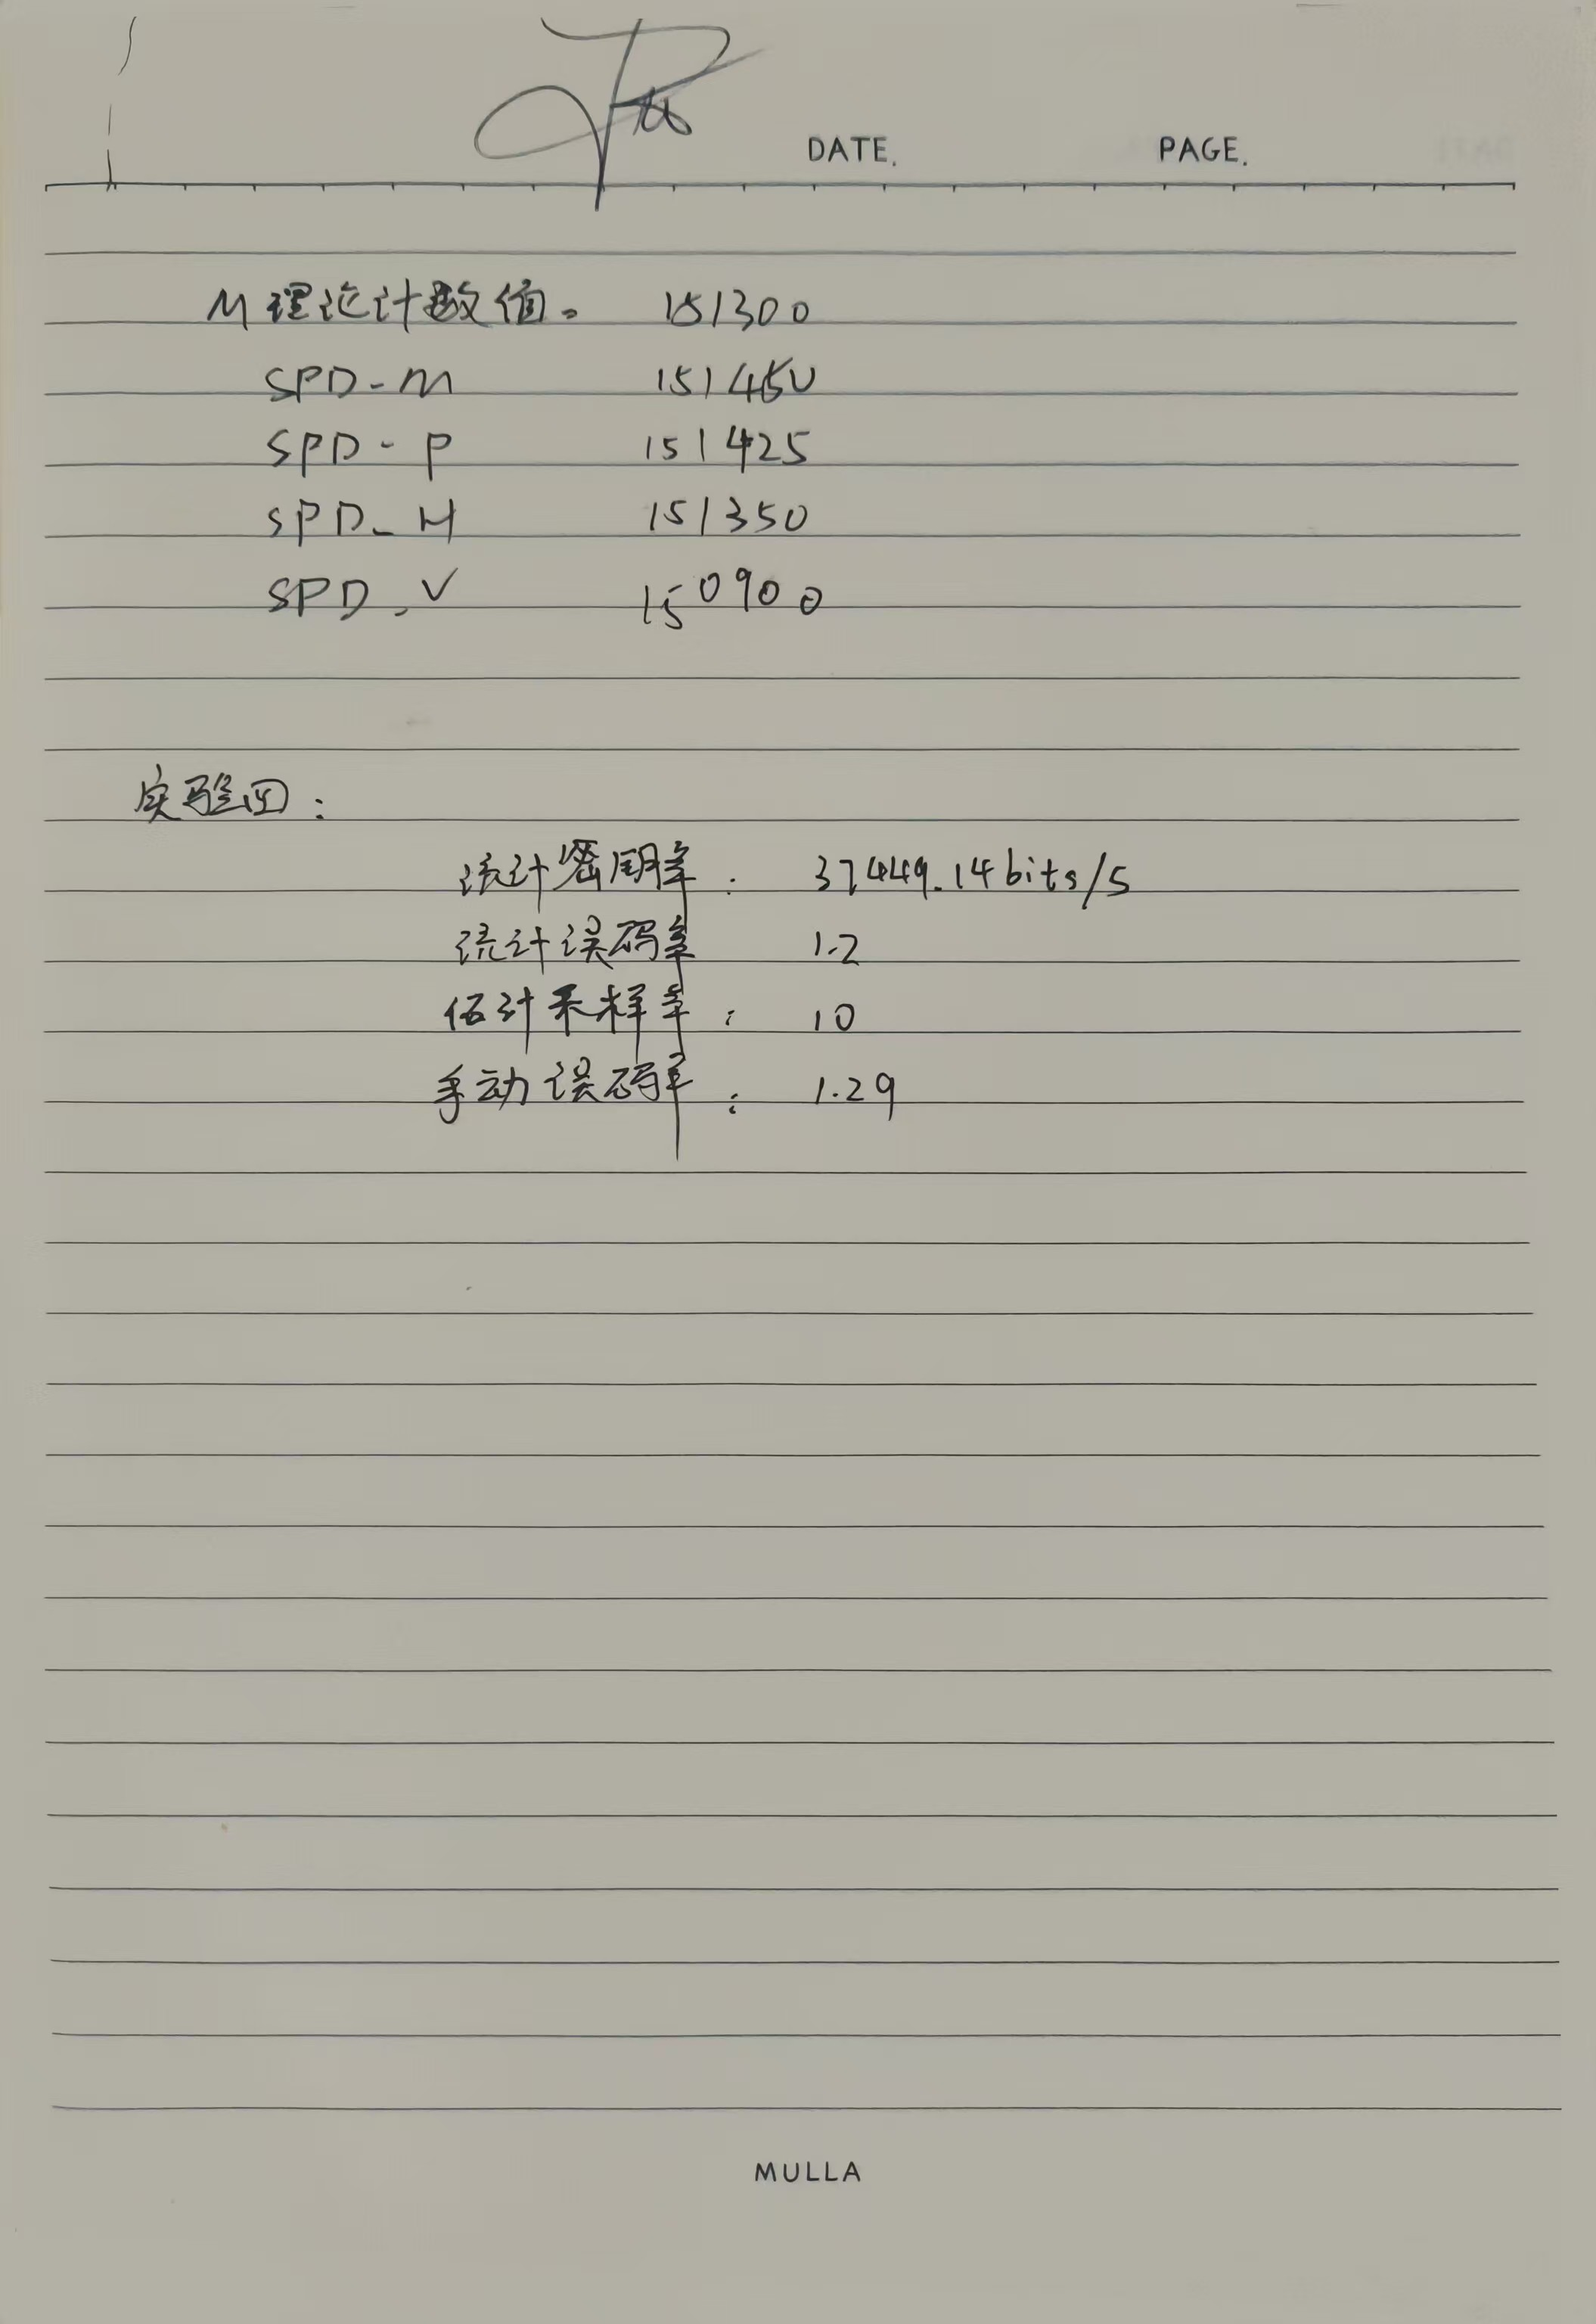
\includegraphics[width=0.3\textwidth]{D3-OriginalData-5.jpg}\label{fig:data5}}
	% 	\caption{原始数据}
	% 	\label{fig:data}
	% \end{figure}
	



%\subsection{原始数据记录}


% \clearpage

	

\clearpage
\begin{table}
	\renewcommand\arraystretch{1.7}
	\begin{tabularx}{\textwidth}{|X|X|X|X|}
	\hline
	专业:& 物理学 &年级:& 2022级\\
	\hline
	姓名: & 戴鹏辉 & 学号:& 22344016\\
	\hline
    日期:& 2024/ & 评分: &\\
	\hline
	\end{tabularx}
\end{table}

\section{D8 \quad 氦氖激光综合实验 \quad\heiti 分析与讨论}

\subsection{实验数据分析}


% 	\subsubsection{实验一 \quad 光的偏振的测量和控制}

		





% 	\subsubsection{实验二 \quad 单光子的探测及相应探测器效率的测量}

		

% 	\subsubsection{实验三 \quad 单光子的标定}




% 	\subsubsection{实验四 \quad 密钥分发过程数据处理}


		

	
% \subsection{实验后思考题}

% % 思考题1
% \begin{question}
% 	是否可以通过直接衰减任意的光源(比如白炽灯)的强度到单光子级别来得到真正的单光子源?(真正的单光子源是指每次触发可以确定性的得到一个仅包含一个光子的光脉冲信号)
% \end{question}

	





% % 思考题2
% \begin{question}
% 	了解单光子探测器暗计数的原理,并设计实验装置测量探测器的暗计数率。
% \end{question}


	





% % 思考题3
% \begin{question}
% 	量子密钥分发实验中对基后的数据,为什么会有误码出现,如何降低误码?
% \end{question}

	
		

\clearpage
\section{D8 \quad 氦氖激光综合实验 \quad\heiti 实验总结}

	\subsection{实验分工}

		

	\subsection{实验心得}

	


\end{document}
